\documentclass[a0paper,portrait]{baposter}

\usepackage{relsize}			% For \smaller.
\usepackage[utf8]{inputenc}		% Use UTF-8.
\usepackage{hyperref}			% Use hyperlinks for emails.
\usepackage{multirow}			% Use tables.
\usepackage{lipsum}
\usepackage{tikz} 				% Use TikZ drawing.
\usepackage{pgfplots} 			% Use plots.
\usepackage{amsmath}        % extensions for typesetting of math
\usepackage{amsfonts}       % math fonts
\usepackage{amsthm}         % theorems, definitions, etc.
\usepackage{enumitem}         % remove list indent

\usetikzlibrary{shapes,matrix,chains,positioning,decorations.pathreplacing,arrows,hobby,decorations.markings,backgrounds}       % more libs

%%% Global Settings %%%%%%%%%%%%%%%%%%%%%%%%%%%%%%%%%%%%%%%%%%%%%%%%%%%%%%%%%%%

\graphicspath{{img/}}	% Root directory of the pictures 
\tracingstats=2			% Enabled LaTeX logging with conditionals

%%% Color Definitions %%%%%%%%%%%%%%%%%%%%%%%%%%%%%%%%%%%%%%%%%%%%%%%%%%%%%%%%%

\definecolor{bordercol}{HTML}{E4E4E4}
\definecolor{headercol1}{HTML}{FD2020}
\definecolor{headercol2}{HTML}{F88A36}
\definecolor{headerfontcol}{RGB}{255,255,255}
\definecolor{boxcolor}{HTML}{FFFFFF}
\definecolor{bgcolor}{HTML}{F0F0F0}

%%%%%%%%%%%%%%%%%%%%%%%%%%%%%%%%%%%%%%%%%%%%%%%%%%%%%%%%%%%%%%%%%%%%%%%%%%%%%%%%
%%% Utility functions %%%%%%%%%%%%%%%%%%%%%%%%%%%%%%%%%%%%%%%%%%%%%%%%%%%%%%%%%%

%%% Delete this before production.
\newcommand*{\todo}{\textbf{TODO}}

%%% Save space in lists. Use this after the opening of the list %%%%%%%%%%%%%%%%
\newcommand{\compresslist}{
	\setlength{\itemsep}{1pt}
	\setlength{\parskip}{0pt}
	\setlength{\parsep}{0pt}
}

%%%%%%%%%%%%%%%%%%%%%%%%%%%%%%%%%%%%%%%%%%%%%%%%%%%%%%%%%%%%%%%%%%%%%%%%%%%%%%%
%%% Document Start %%%%%%%%%%%%%%%%%%%%%%%%%%%%%%%%%%%%%%%%%%%%%%%%%%%%%%%%%%%%
%%%%%%%%%%%%%%%%%%%%%%%%%%%%%%%%%%%%%%%%%%%%%%%%%%%%%%%%%%%%%%%%%%%%%%%%%%%%%%%

\begin{document}
\typeout{Poster rendering started}

\background{
	\begin{tikzpicture}[remember picture,overlay]
		\fill[bgcolor] (-100,-100) rectangle (100,29.7);
		\draw[bordercol] (-100,29.7) -- (100,29.7);
	\end{tikzpicture}
}

%%% General Poster Settings %%%%%%%%%%%%%%%%%%%%%%%%%%%%%%%%%%%%%%%%%%%%%%%%%%%
%%%%%% Eye Catcher, Title, Authors and University Images %%%%%%%%%%%%%%%%%%%%%%
\begin{poster}{
	grid=false,
	% Option is left on true though the eyecatcher is not used. The reason is
	% that we have a bit nicer looking title and author formatting in the headercol
	% this way
	%eyecatcher=false, 
	borderColor=bordercol,
	headerColorOne=headercol2,
	headerColorTwo=headercol2,
	headerFontColor=headerfontcol,
	colspacing=1.5em,
	% Only simple background color used, no shading, so boxColorTwo isn't necessary
	boxColorOne=boxcolor,
	headerfont=\Large\bf\fontfamily{lmss}\selectfont,
	textborder=rectangle,
	background=user,
	bgColorOne=bgcolor,
	headerborder=open,
	headershape=rectangle,
	boxshade=plain,
	linewidth=0.1pt,
	headerheight=130pt
}
%%% Eye Cacther %%%%%%%%%%%%%%%%%%%%%%%%%%%%%%%%%%%%%%%%%%%%%%%%%%%%%%%%%%%%%%%
{
	Eye Catcher, empty if option eyecatcher=false - unused
}
%%% Title %%%%%%%%%%%%%%%%%%%%%%%%%%%%%%%%%%%%%%%%%%%%%%%%%%%%%%%%%%%%%%%%%%%%%
{\bf\fontfamily{lmss}\selectfont
	Genetic Programming in Swift\\
	for Human-competitive Evolution
}
%%% Authors %%%%%%%%%%%%%%%%%%%%%%%%%%%%%%%%%%%%%%%%%%%%%%%%%%%%%%%%%%%%%%%%%%%
{
	\vspace{1em} Petr Mánek, supervisor: František Mráz\\
	{\smaller Faculty of Mathematics and Physics, Charles University in Prague}
}
%%% Logo %%%%%%%%%%%%%%%%%%%%%%%%%%%%%%%%%%%%%%%%%%%%%%%%%%%%%%%%%%%%%%%%%%%%%%
{
	
\includegraphics[width=9em,height=9em]{logo}
}

\begin{posterbox}[name=objectives,column=0]{Objectives}
	\begin{enumerate}[leftmargin=*]
		\compresslist
		\item Implement a genetic programming library in the Swift programming language.
		\item Demonstrate the usage of the library by applying it to sample problems.
	\end{enumerate}
\end{posterbox}

\begin{posterbox}[name=intro-ga,column=0,below=objectives]{Genetic Algorithms}
\lipsum[2]
\end{posterbox}

\begin{posterbox}[name=intro-swift,column=0,below=intro-ga]{Swift Programming Language}
	The Swift programming language has been unveiled in 2014 by the Apple Corporation. Since then, it has been widely adopted by software developers and computer engineers, succeeding Objective-C as the main programming language used for application development on the Apple mobile device platform. Building on proven coding paradigms, such as generics and strongly-typed objects, Swift strives to be a modern, concise and safe alternative to popular languages like Python or C++ while attempting to maintain comparable performance in terms of computational speed and memory management.
\end{posterbox}

\begin{posterbox}[name=arch,column=1]{Architecture}
\lipsum[4]
\end{posterbox}

\begin{posterbox}[name=props,column=1,below=arch]{Properties}
\lipsum[5]
\end{posterbox}

\begin{posterbox}[name=car,column=1,below=props]{Self-driving Car}
	\lipsum[6]
	\begin{center}
		\resizebox {\columnwidth} {!} {
			\begin{tikzpicture}[framed,background rectangle/.style={fill=black!60!green}]
				\draw[
				  black!10!white,
				  line width=3mm,
				  postaction={
				    decorate,
				    decoration={
				      markings,
				      mark=between positions 0 and 1 step 0.2 with
				      {
				        \node[transform shape] {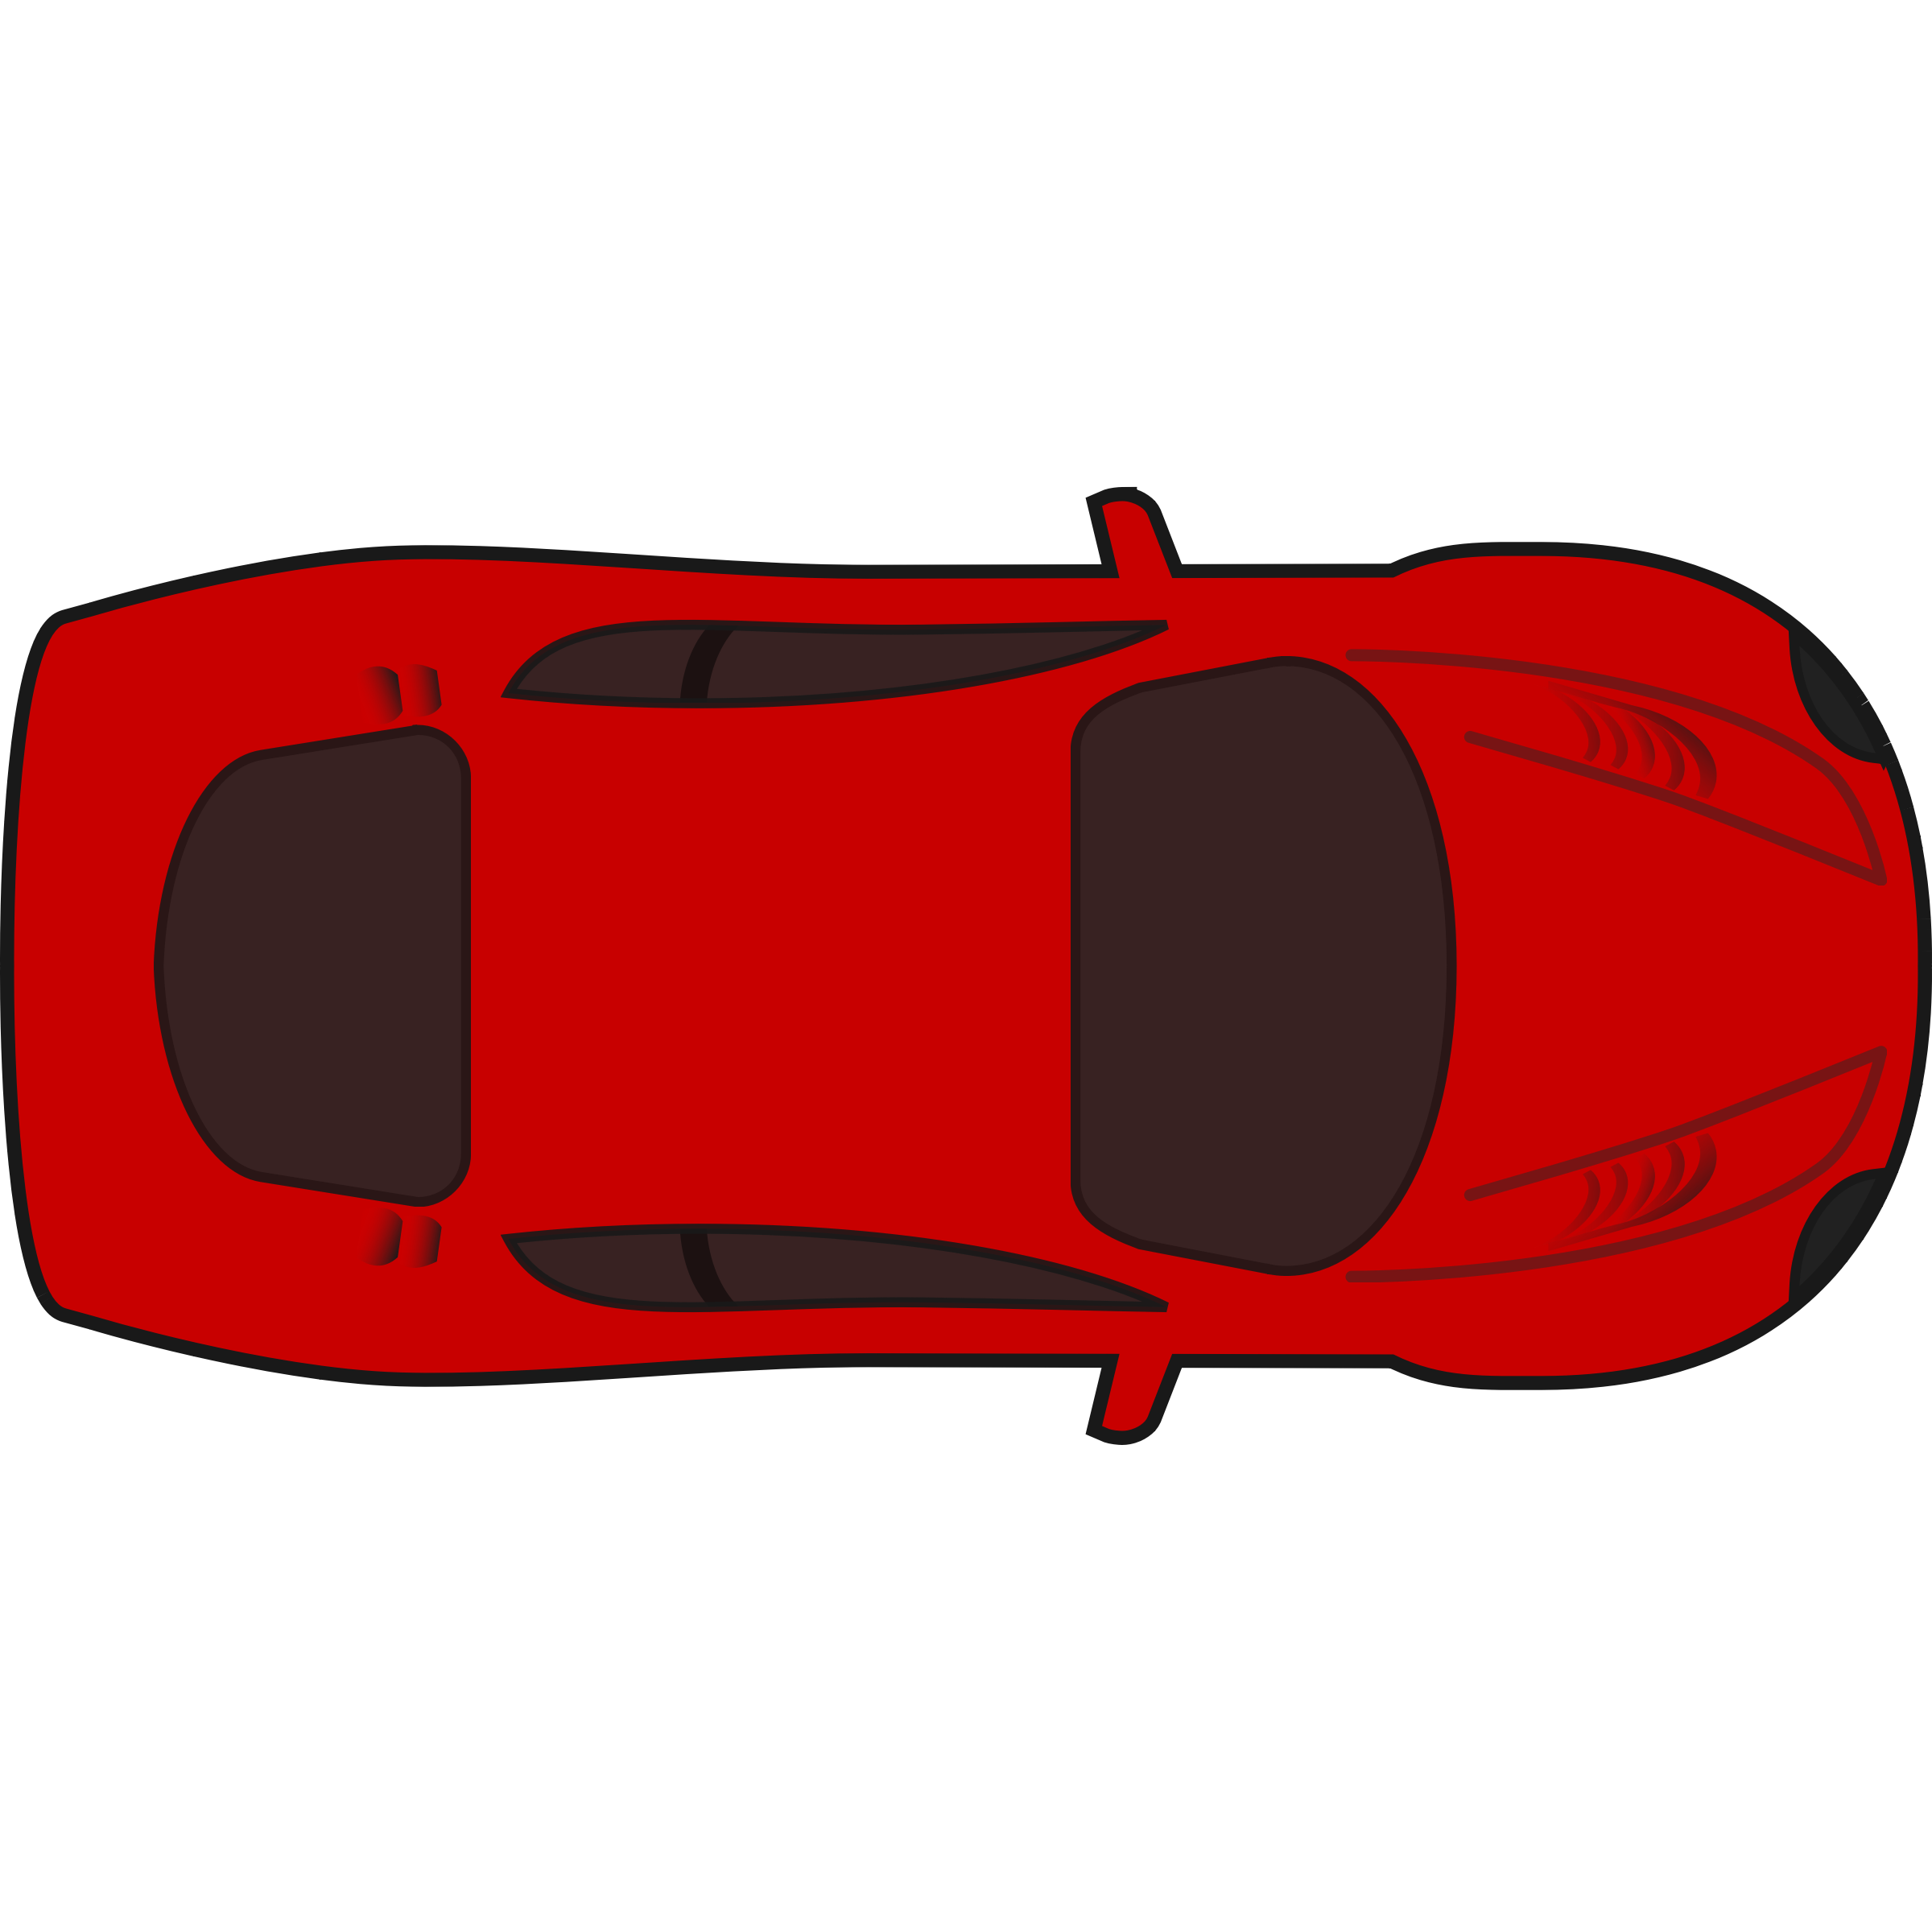
\includegraphics[width=.5cm]{car}};
				      }
				    }
				  }
				]
				(0,0) to[out angle=0,in angle=180,curve through={(1,.4) .. (5,0) .. (10,.5) .. (7,4.3) .. (3,4) .. (1,2)}] (0,0);
			\end{tikzpicture}
		}
	\end{center}
\end{posterbox}

	\begin{posterbox}[name=qwop,column=2]{QWOP Player}
	QWOP is a popular online game, in which the player drives an athlete to finish a 100-meter sprint race as fast as possible. QWOP's difficulty is caused by its control scheme, which only allows the player to move the athlete by contracting individual muscle groups within his body. The challenge of the game is in that sense comparable to the problem of evolving bipedal gaits in physical robots.

	\vspace{0.5em}

	\parbox[c]{0.49\linewidth}{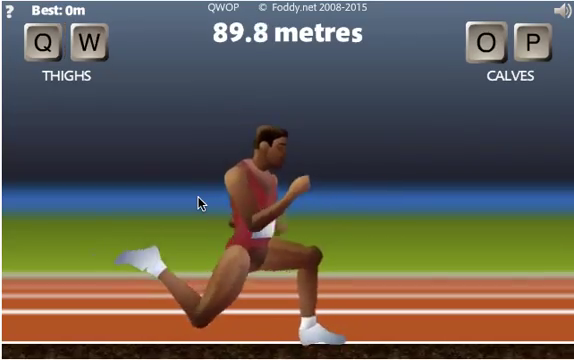
\includegraphics[width=\linewidth]{runner1}}
	\hfill
	\parbox[c]{0.49\linewidth}{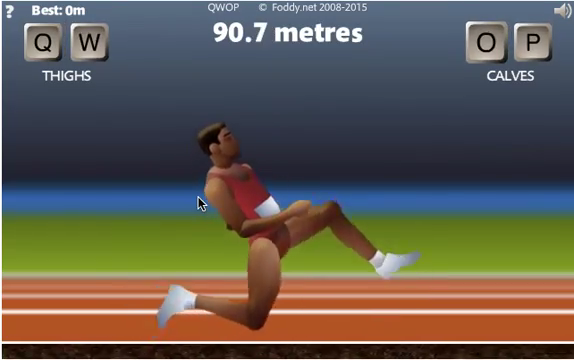
\includegraphics[width=\linewidth]{runner2}}

	\vspace{0.5em}

	The presented library was used to evolve an artificial QWOP player and partially replicate human-competitive results achieved by \todo. In every generation, 80 game strategies were generated and encoded as simple programs (genotype strings), then evaluated by the fitness function

	\vspace{-1.7em}

	\begin{align*}
		f(d_1,d_2,\dots,d_n) = \frac{1}{100n} \sum_{i=1}^n d_i
	\end{align*}

	\vspace{-0.5em}

	where $d_1,d_2,\dots,d_n$ are the distances achieved in $n$ trial 30-second runs. The best strategy after 38 generations was able to complete the race in approximately 152 seconds.

	\vspace{-1.4em}

	\begin{center}
		\resizebox {\columnwidth} {!} {
			\begin{tikzpicture}
				\begin{axis}[
					height=5cm,
					width=9cm,
					grid=major,
					xlabel={Generation},
					ymin=0, ymax=0.3,
					xmin=1, xmax=38,
					no markers,
					legend style={legend pos=north west,font=\small},
					xtick={0,5,10,15,20,25,30,35,38},
					ytick={0,0.1,0.2,...,0.3},
			        yticklabel style={font=\small,xshift=-0.4ex},
			        xticklabel style={font=\small,yshift=-0.5ex},
			        xlabel style={font=\small,xshift=1.0ex}
				]
					
				\addplot table {data/qwop-fitness-best.dat};
				\addlegendentry{Best fitness}

				\addplot table {data/qwop-fitness-average.dat};
				\addlegendentry{Average fitness}

				\end{axis}
			\end{tikzpicture}
		}
	\end{center}
\end{posterbox}

\begin{posterbox}[name=conclusion,column=2,below=qwop]{Conclusions}
\lipsum[8]
\end{posterbox}

\begin{posterbox}[name=ref,column=2,below=conclusion]{References}
\lipsum[9]
\end{posterbox}

\end{poster}
\end{document}
